\documentclass[12pt, fleqn]{article}\usepackage[]{graphicx}\usepackage[]{color}
% maxwidth is the original width if it is less than linewidth
% otherwise use linewidth (to make sure the graphics do not exceed the margin)
\makeatletter
\def\maxwidth{ %
  \ifdim\Gin@nat@width>\linewidth
    \linewidth
  \else
    \Gin@nat@width
  \fi
}
\makeatother

\definecolor{fgcolor}{rgb}{0.345, 0.345, 0.345}
\newcommand{\hlnum}[1]{\textcolor[rgb]{0.686,0.059,0.569}{#1}}%
\newcommand{\hlstr}[1]{\textcolor[rgb]{0.192,0.494,0.8}{#1}}%
\newcommand{\hlcom}[1]{\textcolor[rgb]{0.678,0.584,0.686}{\textit{#1}}}%
\newcommand{\hlopt}[1]{\textcolor[rgb]{0,0,0}{#1}}%
\newcommand{\hlstd}[1]{\textcolor[rgb]{0.345,0.345,0.345}{#1}}%
\newcommand{\hlkwa}[1]{\textcolor[rgb]{0.161,0.373,0.58}{\textbf{#1}}}%
\newcommand{\hlkwb}[1]{\textcolor[rgb]{0.69,0.353,0.396}{#1}}%
\newcommand{\hlkwc}[1]{\textcolor[rgb]{0.333,0.667,0.333}{#1}}%
\newcommand{\hlkwd}[1]{\textcolor[rgb]{0.737,0.353,0.396}{\textbf{#1}}}%
\let\hlipl\hlkwb

\usepackage{framed}
\makeatletter
\newenvironment{kframe}{%
 \def\at@end@of@kframe{}%
 \ifinner\ifhmode%
  \def\at@end@of@kframe{\end{minipage}}%
  \begin{minipage}{\columnwidth}%
 \fi\fi%
 \def\FrameCommand##1{\hskip\@totalleftmargin \hskip-\fboxsep
 \colorbox{shadecolor}{##1}\hskip-\fboxsep
     % There is no \\@totalrightmargin, so:
     \hskip-\linewidth \hskip-\@totalleftmargin \hskip\columnwidth}%
 \MakeFramed {\advance\hsize-\width
   \@totalleftmargin\z@ \linewidth\hsize
   \@setminipage}}%
 {\par\unskip\endMakeFramed%
 \at@end@of@kframe}
\makeatother

\definecolor{shadecolor}{rgb}{.97, .97, .97}
\definecolor{messagecolor}{rgb}{0, 0, 0}
\definecolor{warningcolor}{rgb}{1, 0, 1}
\definecolor{errorcolor}{rgb}{1, 0, 0}
\newenvironment{knitrout}{}{} % an empty environment to be redefined in TeX

\usepackage{alltt}
\usepackage{amsmath}
\usepackage{amssymb}
\usepackage{geometry}
\usepackage{graphicx}
\usepackage{bm}
\usepackage{url}
\usepackage{hyperref}
\usepackage{enumerate}
\usepackage{fullpage}
\IfFileExists{upquote.sty}{\usepackage{upquote}}{}
\begin{document}
\setlength\parindent{0pt}

Lecture 14: Simple Linear Regression\\ 
Practice Problems\\ 
STAT 630, Fall 2020\\

Data was collected on the highway miles per gallon (MPG) and weight (pounds) of 93 cars in the USA in 1993.  Below is some R output for fitting a simple linear regression model to this data.  A scatter plot with the least squares line is also shown below.
\begin{verbatim}
> library(MASS)
> lm1 <- lm(MPG.highway ~ Weight, data=Cars93)
> summary(lm1)

Coefficients:
              Estimate Std. Error t value Pr(>|t|)    
(Intercept) 51.6013654  1.7355498   29.73   <2e-16 ***
Weight      -0.0073271  0.0005548  -13.21   <2e-16 ***
---
Signif. codes:  0 ‘***’ 0.001 ‘**’ 0.01 ‘*’ 0.05 ‘.’ 0.1 ‘ ’ 1

Residual standard error: 3.139 on 91 degrees of freedom
Multiple R-squared:  0.6572,	Adjusted R-squared:  0.6534 
F-statistic: 174.4 on 1 and 91 DF,  p-value: < 2.2e-16
\end{verbatim}

\begin{verbatim}
# make scatter plot with least squares line
> plot(Cars93$Weight, Cars93$MPG.highway, 
    xlab = "Weight (lbs)", ylab = "Highway MPG")
> abline(lm1)
\end{verbatim}

\begin{figure}[ht!]
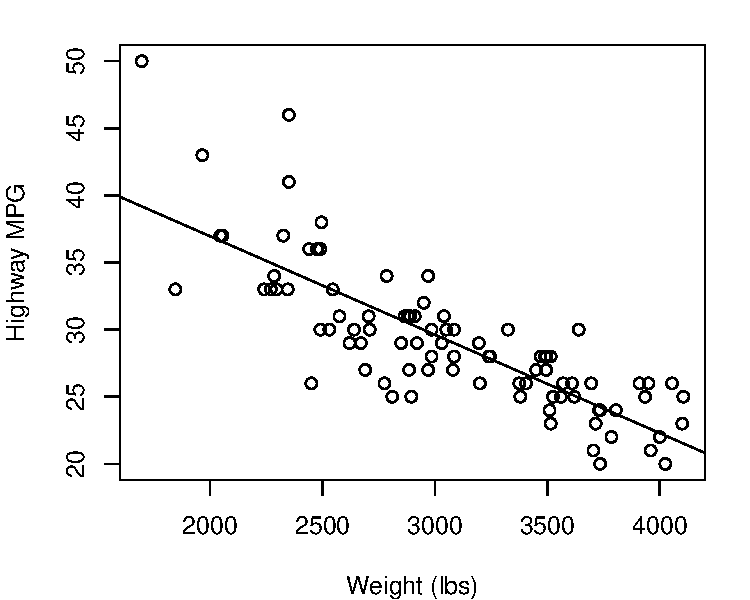
\includegraphics[scale=0.65]{figure/mpg_scatter_fit.pdf}
\end{figure} 
\clearpage

\begin{enumerate}[(a)]
\item Describe the association between weight and highway MPG.\\
\vspace{0.5cm}

\item What are the explanatory and response variables for the linear regression model?\\
\vspace{1cm}

\item Write the equation for the least squares line.\\
\vspace{1cm}

\item Interpret the slope of the model.\\
\vspace{1.75cm}

\item Interpret the intercept of the model, or explain why it does not make sense to try to interpret the intercept.\\
\vspace{1.75cm}

\item What is the predicted highway MPG for a car that weights 3000 pounds?\\
\vspace{1cm}

\item One of car models (BMW 535i) in the data set has an observed weight of 3640 and highway MPG of 30.  Calculate the residual for this car model?\\
\vspace{1.75cm}

\item Interpret the coefficient of determination ($R^2$).\\
\end{enumerate}

\end{document}
